
\newcommand\X{40pt}
\newcommand\Y{-40pt}

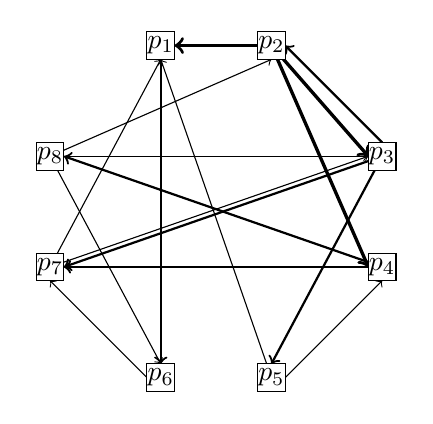
\begin{tikzpicture}

  \draw[thick, ->] (\X, 0)--(\X, 5+3*\Y); %% p1 p6
  \draw[very thick, ->] (-5+2*\X, 0)--(5+\X, 0); %% p2 p1
  \draw[very thick, ->] (2*\X, 0) -- (-5+3*\X, \Y); %% p2 p3
  \draw[very thick, ->] (2*\X, 0) -- (-5+3*\X, 2*\Y); %% p2 p4
  \draw[thick, ->] (3*\X, 5+\Y) -- ( 5+2*\X, 0); %% p3 p2
  \draw[thick, ->] (3*\X, \Y) -- (5pt, 2*\Y); %% p3 p7
  \draw[thick, ->] (3*\X, \Y) -- (2*\X, 5+3*\Y); %% p3 p5
  \draw[thick, ->] (3*\X, 2*\Y) -- (5pt, 2*\Y); %% p4 p7
  \draw[thick, ->] (3*\X, 2*\Y) -- (5pt, \Y); %% p4 p8
  \draw[->] (2*\X, 3*\Y) -- (\X, -5pt); %% p5 p1
  \draw[->] (5+2*\X, 3*\Y) -- (3*\X, -5+ 2*\Y); %% p5 p4
  \draw[->] (-5+\X, 3*\Y) -- (0pt, -5+2*\Y); %% p6 p7
  \draw[->] (0pt, 2*\Y) -- (-5+3*\X, \Y); %% p7 p3
  \draw[->] (0pt, 2*\Y) -- (\X, -5pt); %% p7 p1
  \draw[->] (0pt, \Y) -- (2*\X, -5pt); %% p8 p2
  \draw[->] (0pt, \Y) -- (\X, 5+3*\Y); %% p8 p6
  \draw[->] (0pt, \Y) -- (-5+3*\X, \Y); %% p8 p3
  
  \draw[fill=white] (\X, 0)node{$p_1$}+(-5pt, -5pt)rectangle+(5pt, 5pt);
  \draw[fill=white] (2*\X, 0)node{$p_2$}+(-5pt, -5pt)rectangle+(5pt, 5pt);
  \draw[fill=white] (3*\X, \Y)node{$p_3$}+(-5pt, -5pt)rectangle+(5pt, 5pt);
  \draw[fill=white] (3*\X, 2*\Y)node{$p_4$}+(-5pt, -5pt)rectangle+(5pt, 5pt);
  \draw[fill=white] (2*\X, 3*\Y)node{$p_5$}+(-5pt, -5pt)rectangle+(5pt, 5pt);
  \draw[fill=white] (1*\X, 3*\Y)node{$p_6$}+(-5pt, -5pt)rectangle+(5pt, 5pt);
  \draw[fill=white] (0 , 2*\Y)node{$p_7$}+(-5pt, -5pt)rectangle+(5pt, 5pt);
  \draw[fill=white] (0 , \Y)node{$p_8$}+(-5pt, -5pt)rectangle+(5pt, 5pt);


\end{tikzpicture}